\subsubsection{AMS1117}

El módulo \texttt{AMS1117} es un regulador de voltaje de $5 V$, el cual se utiliza para alimentar el microcontrolador. Es un regulador lineal de bajo \textit{drop-out} utilizado para suavizar la alimentación del microcontrolador. 

En su hoja de características indica que (en nuestra versión) tiene una tensión de salida fija de $5 V$, un \textit{drop-out} mínimo de $1.3 V$ en el peor caso, una regulación de línea de hasta $10 mV$ para nuestra tensión de entrada y salida diseñadas, regulación de carga de hasta $35 mV$ y una corriente máxima de $0.9 A$ \cite{advancedmonolithicsystemsAMS1117}.

Utilizaremos el regulador a la salida del regulador reductor, con la finalidad de suavizar los picos de tensión que aparecen por la naturaleza conmutada de dicho regulador.

\begin{figure}[H]
    \centering
    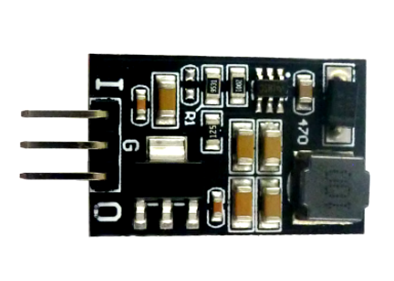
\includegraphics[width=0.5\textwidth]{images/2-hardware/componentes/AMS1117.png}
    \caption{\texttt{LDO AMS1117}}
    \label{fig:hardware/modulos/ldo-ams1117}
\end{figure}

En la \autoref{fig:hardware/modulos/ldo-picos} se puede ver que la tensión de salida del regulador presenta picos de aproximadamente $110\ mV$, que se eliminan gracias a este componente. Aparece en la tensión de salida de este componente una oscilación de $20\ mV$, por lo que se ha reducido significativamente.

\begin{figure}[H]
    \centering
    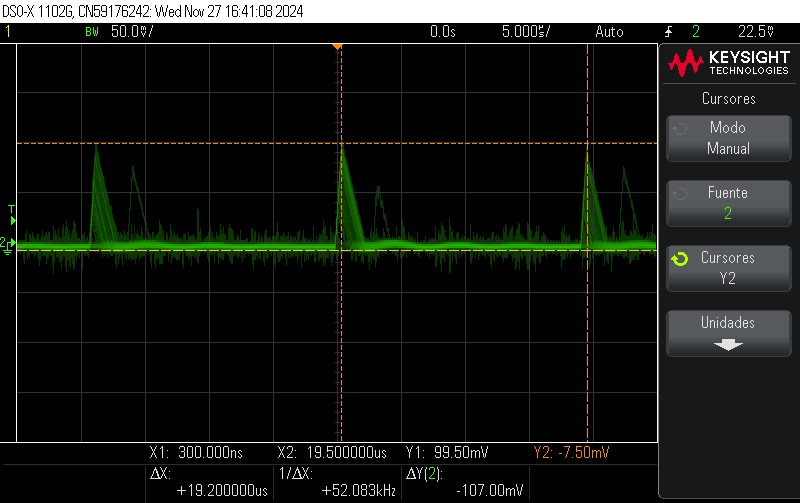
\includegraphics[width=0.5\textwidth]{images/2-hardware/componentes/ldo/picosSinLDO.jpg}
    \caption{Componente alterna de la tensión de salida del regulador conmutado}
    \label{fig:hardware/modulos/ldo-picos}
\end{figure}

\begin{figure}[H]
    \centering
    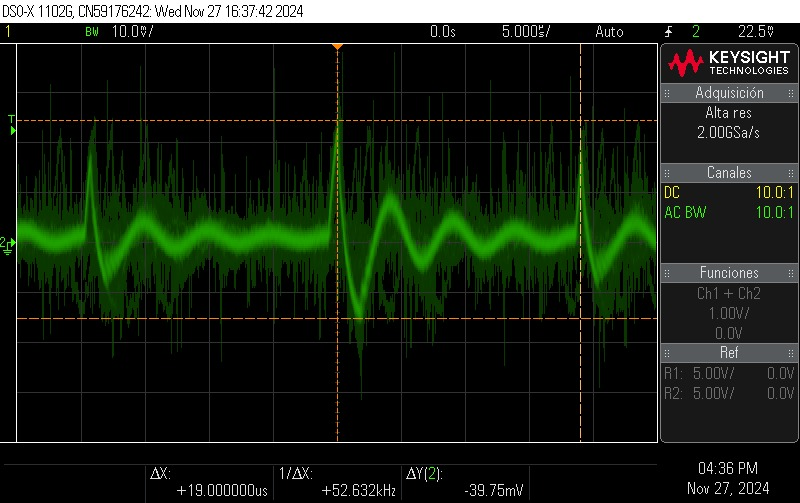
\includegraphics[width=0.5\textwidth]{images/2-hardware/componentes/ldo/picosConLDO.jpg}
    \caption{Componente alterna de la tensión de salida del LDO}
    \label{fig:hardware/modulos/ldo-sin-picos}
\end{figure}

Experimentalmente, hemos comprobado que la tensión de salida no converge hacia los $5\ V$ anunciados para tensiones menores de $6.7\ V$, por lo que el \textit{drop-out} es ligeramente superior al especificado. Sin embargo, como lo alimentamos con un regulador conmutado regulable no es ningún problema, solamente incrementa ligeramente la disipación de potencia del regulador.

En la caracterización, se han medido dos valores: \begin{itemize}
    \item Regulación de línea: Se han medido valores de tensión de salida variando la tensión de entrada, obteniendo el siguiente valor: \[ \text{Reg. Línea} \equiv \frac{\Delta V_o}{\Delta V_i} = \frac{V_{o2} - V_{o1}}{V_{i2} - V_{i1}} = \frac{5.00376 - 5.00372}{8 - 7.2} = 50\ \mu V/V \]

    \item Regulación de carga: Se han aplicado distintas resistencias a la salida del regulador y se ha medido la variación de la tensión de salida en función de dicha carga: \[ \text{Reg. Carga} \equiv \frac{\Delta V_o}{\Delta I_o} = \frac{V_{o2} - V_{o1}}{I_{o2} - I_{o1}} = \frac{V_{o2} - V_{o1}}{\frac{V_{o2}}{R_2} - \frac{V_{o1}}{R_1}} = \frac{5.00345 - 5.00262}{5.00345/900 - 5.00262/100} = -18.67\ mV/A \]
\end{itemize}